\documentclass{article}
\renewcommand{\baselinestretch}{1.25}

\usepackage{xeCJK}  % support character

% monokai code
\usepackage{color}
\definecolor{bg}{rgb}{0.152941, 0.156863, 0.133333} 
\usepackage{minted}
\usemintedstyle{monokai}

% insert images
\usepackage{graphicx}
\graphicspath{{images/}{../images/}}
\usepackage{amsmath}
\numberwithin{figure}{section}
\numberwithin{table}{section}
\numberwithin{listing}{section}

\usepackage{subcaption}

% hyperlink
\usepackage{hyperref}

\usepackage{multirow}

\author{郭一隆(2013011189)}
\title{图像处理实验报告}

\begin{document}
    \maketitle

    \tableofcontents
    \newpage

    \listoffigures
    \listoftables
    \newpage

    \renewcommand\listoflistingscaption{List of source codes}
    \listoflistings
    \newpage

    \section{基础知识} % (fold)
    \label{sec:基础知识}

        在\texttt{MATLAB}中,像素值用\texttt{uint8}类型表示,参与浮点数运算前需要转成\texttt{double}型。Section \ref{sec:基础知识} 中“测试图像”指的是\href{run:../resource/hall.mat}{\texttt{hall.mat}}中的\textbf{彩色图像}。

        \begin{enumerate}
            \item \texttt{MATLAB}提供了图像处理工具箱,在命令窗口输入\texttt{help images}可查看该工具箱内的所有函数。请阅读并大致了解这些函数的基本功能。

                \begin{table}[H]
                    \caption{图像处理工具箱函数概览(部分)}
                    \label{tab:help_images}
                    \centering
                
                    \begin{tabular}{l|l}
                    \hline
                
                    \hline
                    \textbf{函数名} & \textbf{功能} \\
                    \hline
                        \texttt{im2double} & 将图像像素值转为\texttt{double}型 \\
                    \hline
                        \texttt{imshow} & 在\texttt{figure}中显示图像 \\
                    \hline
                        \texttt{rgb2gray} & 将彩色图像转换为灰度值图像 \\
                    \hline
                        \texttt{imwrite} & 将图像矩阵写入文件 \\
                
                    \hline
                    \end{tabular}
                \end{table}

            \item 利用\texttt{MATLAB}提供的\texttt{Image file I/O}函数分别完成以下处理:
                \begin{enumerate}
                    \item 以测试图像的中心为圆心,图像的长和宽中较小值的一半为半径画一个\textcolor{red}{红颜色}的圆;

                        \textbf{思路:}利用\texttt{meshgrid}函数生成行列索引矩阵\texttt{I, J},将圆内部的像素点标为\textbf{逻辑1},再利用逻辑索引将测试图像圆内的部分替换为\textcolor{red}{红色像素点}。

                        \begin{listing}[H]
                            \caption{\texttt{draw\_circle.m}}
                            \label{listing:draw_circle}
                            \inputminted[bgcolor=bg, linenos, fontsize=\footnotesize]{matlab}{../draw_circle.m}
                        \end{listing}

                        \begin{figure}[H]
                            \centering
                                \begin{subfigure}{0.3\textwidth}
                                    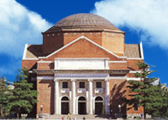
\includegraphics[width=\linewidth]{hall_color}
                                    \caption{处理前}
                                    \label{fig:hall_color}
                                \end{subfigure}

                                \begin{subfigure}{0.3\textwidth}
                                    
\includegraphics[width=\linewidth]{hall_color_red_circle}
                                    \caption{处理后}
                                    \label{fig:hall_color_red_circle}
                                \end{subfigure}

                            \caption{在大礼堂中心绘制红圆}
                            \label{fig:red_circle}
                        \end{figure}

                    \item 将测试图像涂成国际象棋状的“黑白格”的样子,其中“黑”即黑色,“白”则意味着\textbf{保留原图}。
                \end{enumerate}

                用一种看图软件浏览上述两个图,看是否达到了目标。
        \end{enumerate}
    
    % section 基础知识 (end)

\end{document}